\documentclass[onlytextwidth]{beamer}
\usepackage[utf8]{inputenc}
\usepackage{microtype}
\usepackage{amsmath}
\usepackage{amssymb}
\usepackage[nomessages]{fp} %\FPeval{\var-name}{2*sin(pi/6)}
\usepackage{siunitx} %units in math. eg 20\milli\meter
\usepackage{yhmath} % for arcs, overparenth command
\usepackage{tikz} %graphics
\usetikzlibrary{quotes, angles}
%\usepackage{graphicx} already loaded by beamer class
%consider setting \graphicspath{{images/}}
%\parskip ?? to avoid paragraph indent
\usepackage{multicol} %may not need this package, just columns environment
\usepackage{venndiagram}

\subtitle[BECA]{Bronx Early College Academy}
\author[Huson]{Christopher J. Huson PhD}

\setbeamertemplate{headline}{\vskip2mm 
  BECA / \insertshortauthor \, / \inserttitle
  \hfill 
  \insertsection
  }

\title{Geometry Unit 1: Segments, Length, and Area}
\date{8-23 September 2022}

\begin{document}
\frame{\titlepage}

\section[Outline]{}
\frame{\tableofcontents}

\section{1.1 Segment addition \hfill 8 September}
\begin{frame}{Learning Target: I can measure my world}
  {CCSS: HSG.CO.A.1 Know precise geometric definitions \hfill \alert{1.1 Thursday 8 Sept}}
  \begin{block}{Do Now: Measurement}
    \begin{enumerate}
        \item Diagram people closest to you and their distance
        \item Early finishers: Calculate diagonal distances
        \item (add classroom desk image, diagram, test instructions)
    \end{enumerate}
    \end{block}
    Lesson: Points, line segments, length; Segment addition postulate \\[0.25cm]
    Homework: Write for me your ``math autobiography''
\end{frame}

\begin{frame}{A \emph{diagram} is a simplied image representing a situation}
  {This is an example diagram of a desk arrangement}
  %\includegraphics[]{desk-layout-diagram}
  \begin{block}{When making diagrams}
    Include common elements: labels, titles, distances \par
    \emph{Conventions}: standard ways of doing things to make it easier to work with other people
  \end{block} \vspace{1cm}
  Write down vocabulary and terminology in your notebook with definitions and examples. (e.g. I write important terms in \emph{italics})
\end{frame}

\begin{frame}{Example: Points and line segments}
  Shown points $P$, $A$, $B$, $C$, line segments $\overline{AB}$, $\overline{BC}$
  \vspace{1cm}
  \begin{columns}
    \column{0.7\textwidth}
      \begin{tikzpicture}
      \draw [fill] (5,2) circle [radius=0.05] node[below]{$P$};
      \draw [-, thick] (0,1)--(3,1);
      \draw [fill] (0,1) circle [radius=0.05] node[below]{$A$};
      \draw [fill] (3,1) circle [radius=0.05] node[below]{$B$};
      \draw [-, thick] (3,0)--(7,0);
      \draw [fill] (3,0) circle [radius=0.05] node[below]{$B$};
      \draw [fill] (7,0) circle [radius=0.05] node[below]{$C$};
    \end{tikzpicture}

    \column{0.3\textwidth}
      Given:\par $AB=3$ \par $BC=4$
  \end{columns} \vspace{1cm}
    The \emph{length} of a line segment is the distance between the two end points. The length of segment $\overline{AB}$ is written $AB$ (no bar over).
\end{frame}

\begin{frame}{A number line is useful for calculating length or distance}
  {Take the difference in the points' values}
  Given $\overline{PQ}$ as shown on the number line.
\begin{center}
  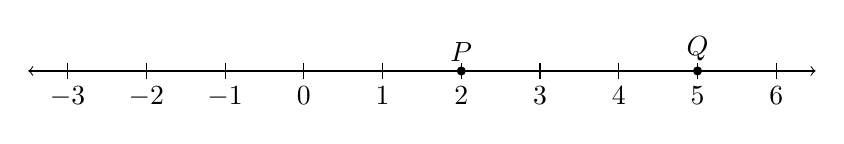
\begin{tikzpicture}
    \draw [<->] (-3.5,0)--(6.5,0);
    \draw [-, thick] (2,0)--(5,0);
    \foreach \x in {-3,...,6} %2 leading for diff!=1
      \draw[shift={(\x,0)},color=black] (0pt,-3pt) -- (0pt,3pt) node[below=5pt]  {$\x$};
      \draw [fill] (2,0) circle [radius=0.05] node[above] {$P$};
      \draw [fill] (5,0) circle [radius=0.05] node[above] {$Q$};
  \end{tikzpicture}
\end{center}
Find the distance on the number line between the points $P$ and $Q$. \vspace{2cm}
\end{frame}

\begin{frame}{Negative number practice on a number line}
  {Take the difference in the points' values. Check by counting the marks.}
  Given $\overline{MN}$ with $M(-1)$ and $N(3)$, as shown on the number line.
\begin{center}
    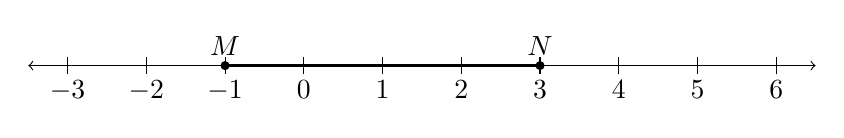
\begin{tikzpicture}
      \draw [<->] (-3.5,0)--(6.5,0);
      \draw [-, thick] (-1,0)--(3,0);
      \foreach \x in {-3,...,6} %2 leading for diff!=1
        \draw[shift={(\x,0)},color=black] (0pt,-3pt) -- (0pt,3pt) node[below=5pt]  {$\x$};
        \draw [fill] (-1,0) circle [radius=0.05] node[above] {$M$};
        \draw [fill] (3,0) circle [radius=0.05] node[above] {$N$};
    \end{tikzpicture}
  \end{center} \bigskip
What is the length of the segment $\overline{MN}$? Show your work as an equation. \par \bigskip
Can a length be a negative number? \vspace{2cm}  
\end{frame}

\begin{frame}{Decimal practice on a number line}
  {Mark the points then take the difference in the points' values.}
  Given $\overline{GH}$ with $G(1)$ and $H(4.5)$. \\[1.5cm]
  \begin{center}
    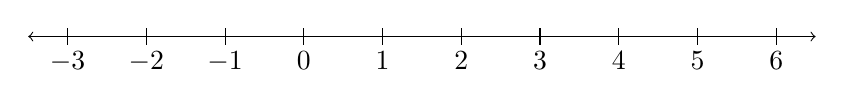
\begin{tikzpicture}
      \draw [<->] (-3.5,0)--(6.5,0);
      %\draw [-, thick] (1,0)--(4.5,0);
      \foreach \x in {-3,...,6} %2 leading for diff!=1
        \draw[shift={(\x,0)},color=black] (0pt,-3pt) -- (0pt,3pt) node[below=5pt]  {$\x$};
        %\draw [fill] (1,0) circle [radius=0.05] node[above] {$M$};
        %\draw [fill] (4.5,0) circle [radius=0.05] node[above] {$N$};
    \end{tikzpicture}
  \end{center}
    \begin{enumerate}
      \item Mark and label the points and segment on the number line.
      \item What is the length of the segment $\overline{GH}$? Show your work as an equation.
    \end{enumerate} \vspace{2cm}  
\end{frame}

\begin{frame}{Take class notes in a composition book}
  {Copy definitions using your own words. Write down example diagrams and problems}
  Definitions: \bigskip
    \begin{description}
      \item[Point] A location, has no size; label with capital letter, $P$
      \item[End point] A point at the end of a line segment
      \item[Segment] Two points and all the points between them; label with \emph{end points} and a bar, e.g. $\overline{AB}$
      \item[Distance] The positive difference between two points on a number line (length is the same thing). $AB=3$ inches
      \item[Conventions] Standard ways of doing things to make it easier to work with other people
    \end{description}
\end{frame}


\begin{frame}{Take class notes in a composition book}
  {Copy definitions using your own words. Write down example diagrams and problems}
    \begin{definition}
      \begin{itemize}
        \item Point A location, has no size; label with capital letter, $P$
        \item End point A point at the end of a line segment
        \item Segment Two points and all the points between them; label with \emph{end points} and a bar, e.g. $\overline{AB}$
        \item Distance The positive difference between two points on a number line (length is the same thing). $AB=3$ inches
        \item Conventions Standard ways of doing things to make it easier to work with other people
      \end{itemize}
    \end{definition}
\end{frame}

\begin{frame}{Absolute value: the distance from a point to the origin}
  {Always a positive number (or zero)}
    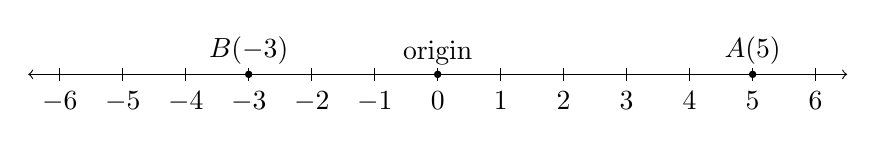
\begin{tikzpicture}[scale=0.8]
      \draw [<->] (-6.5,0)--(6.5,0);
      \foreach \x in {-6,...,6} %2 leading for diff!=1
        \draw[shift={(\x,0)},color=black] (0pt,-3pt) -- (0pt,3pt) node[below=5pt]  {$\x$};
        \draw [fill] (0,0) circle [radius=0.05] node[above] {origin};
        \draw [fill] (5,0) circle [radius=0.05] node[above] {$A(5)$};
        \draw [fill] (-3,0) circle [radius=0.05] node[above] {$B(-3)$};
    \end{tikzpicture} \par \bigskip
    The absolute value of 5 is 5. $|5|=5$ \par \bigskip
    The absolute value of $-3$ is 3. $|-3|=3$
\end{frame}

\section{1.2 Solve for length \hfill 9 September}
\begin{frame}{Learning Target: I can solve for segment lengths}
  {CCSS: HSG.CO.A.1 Know precise geometric definitions  \hfill \alert{1.2 Friday 9 September}}
  Shown \emph{collinear} points $A$, $B$, $C$. Given $AB=3$, $BC=4$. \par
  Find $AC$.
    \begin{center}
      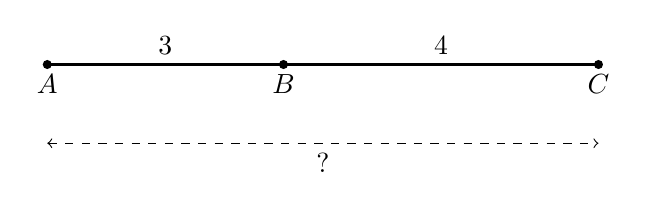
\begin{tikzpicture}
        \draw [fill] (0,0) circle [radius=0.05] node[below]{$A$};
        \draw [-, thick] (0,0)--(7,0);
        \draw [fill] (3,0) circle [radius=0.05] node[below]{$B$};
        \draw [fill] (7,0) circle [radius=0.05] node[below]{$C$};
        \node at (1.5,0) [above]{$3$};
        \node at (5,0) [above]{$4$};
        \draw [<->, dashed] (0,-1)--(7,-1);
        \node at (3.5,-1) [below]{$?$};
      \end{tikzpicture}
    \end{center} \vspace{1cm}
  Definition: Points are \emph{collinear} when they lie on a straight line. \par \medskip
  \emph{Segment Addition Postulate}: lengths add. e.g. $AB+BC=AC$
\end{frame}

\begin{frame}{Example 2: Points and line segments}
  {Segment Addition Postulate}
  Given collinear points $Q$, $R$, $S$, with $QR=11$, $QS=20$. \par \bigskip
  Find $RS$.
  \begin{center}
    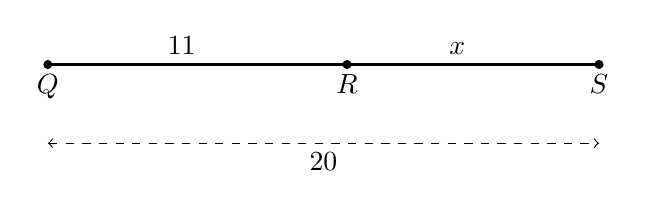
\begin{tikzpicture}
      \draw [fill] (0,0) circle [radius=0.05] node[below]{$Q$};
      \draw [-, thick] (0,0)--(7,0);
      \draw [fill] (3.8,0) circle [radius=0.05] node[below]{$R$};
      \draw [fill] (7,0) circle [radius=0.05] node[below]{$S$};
      \node at (1.7,0) [above]{$11$};
      \node at (5.2,0) [above]{$x$};
      \draw [<->, dashed] (0,-1)--(7,-1);
      \node at (3.5,-1) [below]{$20$};
    \end{tikzpicture}
  \end{center}
  \begin{enumerate}
    \item How would you check your answer?
    \item Which equation represents the situation?
    \begin{columns}[c]
      \column{0.5\textwidth}
      \hspace{2cm} $11 + x = 20$
      \column{0.5\textwidth}
      $x = 20 - 11$
    \end{columns}
  \end{enumerate}
  \end{frame}

\begin{frame}{Example 3: Segment addition postulate}
  Given $\overline{JKL}$, $JK=2x+3$, $KL=5$, $JL=12$. Find ${x}$.
  \begin{center}
    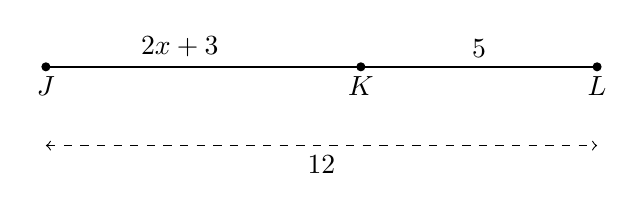
\begin{tikzpicture}
      \draw [-, thick] (0,0)--(7,0);
      \draw [fill] (0,0) circle [radius=0.05] node[below]{$J$};
      \draw [fill] (4,0) circle [radius=0.05] node[below]{$K$};
      \draw [fill] (7,0) circle [radius=0.05] node[below]{$L$};
      \node at (1.7,0) [above]{$2x+3$};
      \node at (5.5,0) [above]{$5$};
      \draw [<->, dashed] (0,-1)--(7,-1);
      \node at (3.5,-1) [below]{$12$};
    \end{tikzpicture}
  \end{center}
  \begin{enumerate}
    \item Write down an equation to represent the situation. \vspace{1cm}
    \item Solve for $x$. \vspace{1cm}
    \item Check your answer.
  \end{enumerate} \vspace{1cm}
\end{frame}

\begin{frame}{Example 3: Use algebra to model a length situation}
  {Write the steps in your notebook}
  Given $\overline{JKL}$, $JK=2x+3$, $KL=5$, $JL=12$. Find ${x}$.
  \begin{center}
    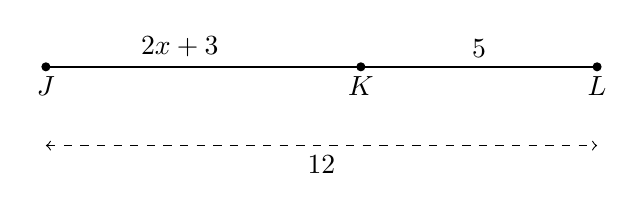
\begin{tikzpicture}
      \draw [-, thick] (0,0)--(7,0);
      \draw [fill] (0,0) circle [radius=0.05] node[below]{$J$};
      \draw [fill] (4,0) circle [radius=0.05] node[below]{$K$};
      \draw [fill] (7,0) circle [radius=0.05] node[below]{$L$};
      \node at (1.7,0) [above]{$2x+3$};
      \node at (5.5,0) [above]{$5$};
      \draw [<->, dashed] (0,-1)--(7,-1);
      \node at (3.5,-1) [below]{$12$};
    \end{tikzpicture}
  \end{center}
\begin{columns}[]{}
  \column{0.4\textwidth}
    \[JK+KL=JL\]
    \[(2x+3)+5=12\]
    \[2x+8=12\]
    \[2x=4\]
    \[x=2\]
    \[2(2)+3+5=12?\]
  \column{0.6\textwidth}
    \begin{enumerate}
        \item Sketch and label the situation
        \item Write a geometric equation
        \item Substitute algebraic values
        \item Solve for $x$
        \item Answer the question
        \item Check your answer
    \end{enumerate}
  \end{columns}
\end{frame}

\begin{frame}{Example 4 (challenge): Segment addition postulate}
  Given $\overline{ABC}$, $AB=3x-7$, $BC=x+5$, $AC=14$. Find ${AB}$.\vspace{1cm}
  \begin{center}
      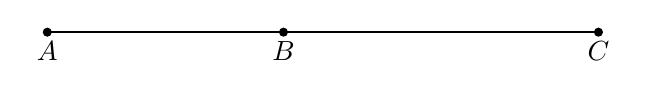
\begin{tikzpicture}
      \draw [-, thick] (0,0)--(7,0);
      \draw [fill] (0,0) circle [radius=0.05] node[below]{$A$};
      \draw [fill] (3,0) circle [radius=0.05] node[below]{$B$};
      \draw [fill] (7,0) circle [radius=0.05] node[below]{$C$};
    \end{tikzpicture}
  \end{center} \vspace{3cm}
  \end{frame}

\begin{frame}{Example 5: Solve an equation with $x$ on both sides}
  Given $\overrightarrow{DEF}$, $DE=x+1$, $EF=9$, $DF=3x$. Find ${DE}$.\vspace{1cm}
  \begin{center}   
  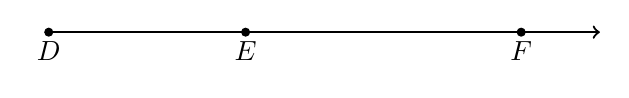
\begin{tikzpicture}
      \draw [->, thick] (0,0)--(7,0);
      \draw [fill] (0,0) circle [radius=0.05] node[below]{$D$};
      \draw [fill] (2.5,0) circle [radius=0.05] node[below]{$E$};
      \draw [fill] (6,0) circle [radius=0.05] node[below]{$F$};
    \end{tikzpicture}
  \end{center} \vspace{3cm}
\end{frame}


\section{1.3 Terminology and notation, 12 September}
\begin{frame}{Learning Target: I can use geometric conventions}
  {CCSS: HSG.CO.A.1 Know precise geometric definitions  \hfill \alert{1.3 Monday 12 Sept}}
  Do Now: Given collinear points $A$, $B$, $C$, with $AB=7$, $AC=13$.
  \begin{center}
    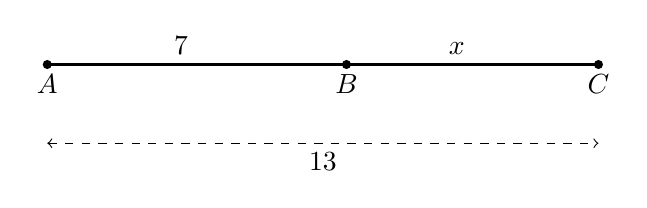
\begin{tikzpicture}
      \draw [fill] (0,0) circle [radius=0.05] node[below]{$A$};
      \draw [-, thick] (0,0)--(7,0);
      \draw [fill] (3.8,0) circle [radius=0.05] node[below]{$B$};
      \draw [fill] (7,0) circle [radius=0.05] node[below]{$C$};
      \node at (1.7,0) [above]{$7$};
      \node at (5.2,0) [above]{$x$};
      \draw [<->, dashed] (0,-1)--(7,-1);
      \node at (3.5,-1) [below]{$13$};
    \end{tikzpicture}
  \end{center}
  \begin{enumerate}
    \item Circle the equation that most simply represents the situation.
    \begin{columns}[c]
      \column{0.5\textwidth}
      $7 + x = 13$
      \column{0.5\textwidth}
      $x = 13 - 7$
    \end{columns}
    \item Find $BC$.
  \end{enumerate}
  \end{frame}

\begin{frame}{Write down an example of each geometric object.}
{Use proper notation.}
  \begin{enumerate}
    \item point
    \item line segment
    \item end point
    \item three collinear points
      \begin{tikzpicture}
      \draw [-, thick] (0,2)--(3,1);
      \draw [fill] (0,2) circle [radius=0.05] node[below]{$R$};
      \draw [fill] (3,1) circle [radius=0.05] node[below]{$S$};
      \draw [-, thick] (5,0)--(8,3);
      \draw [fill] (5,0) circle [radius=0.05] node[above left]{$T$};
      \draw [fill] (7,2) circle [radius=0.05] node[above left]{$U$};
      \draw [fill] (8,3) circle [radius=0.05] node[above left]{$V$};
    \end{tikzpicture}
    \item Given $TU=1.4$, $UV=0.6$. Find $TV$. (label the diagram first)
  \end{enumerate}
\end{frame}

\begin{frame}{More definitions: lines, rays, planes}
  A \emph{line} extends infinitely in both directions, $\overleftrightarrow{AB}$. \par
  (sometimes labeled with a small letter, for example, line $k$)
  \begin{center}
    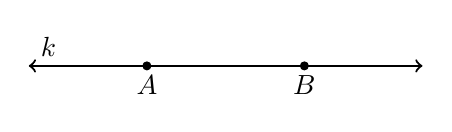
\begin{tikzpicture}
      \draw [<->, thick] (0,1)--(5,1);
      \node at (0.25, 1)[above]{$k$};
      \draw [fill] (1.5,1) circle [radius=0.05] node[below]{$A$};
      \draw [fill] (3.5,1) circle [radius=0.05] node[below]{$B$};
    \end{tikzpicture}
  \end{center}
    A \emph{ray} has one end point and extends infinitely in one direction, $\overrightarrow{CD}$.
    \begin{center}
    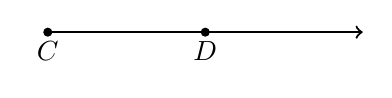
\begin{tikzpicture}
      \draw [->, thick] (3,0)--(7,0);
      \draw [fill] (3,0) circle [radius=0.05] node[below]{$C$};
      \draw [fill] (5,0) circle [radius=0.05] node[below]{$D$};
      \end{tikzpicture}
    \end{center}
    A \emph{plane} is flat and extends infinitely in two directions, $p$.
    \begin{center}
      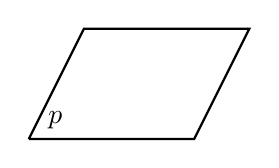
\begin{tikzpicture}[scale=0.7]
      \draw [thick](0,0) node[above right]{$\ p$} --(3,0)--(4,2)--(1,2)--(0,0);
    \end{tikzpicture}
  \end{center}
\end{frame}

\begin{frame}{Several objects are shown in a plane}
  \begin{enumerate}
    \item T \quad F \quad The name of the plane is $m$
    \item T \quad F \quad The line $\overleftrightarrow{WY}$ is in the plane
    \item T \quad F \quad The ray $\overrightarrow{WX}$ is shown in the plane
    \item T \quad F \quad Points $W$, $X$, and $Z$ are collinear
    \end{enumerate}
    \begin{center}
      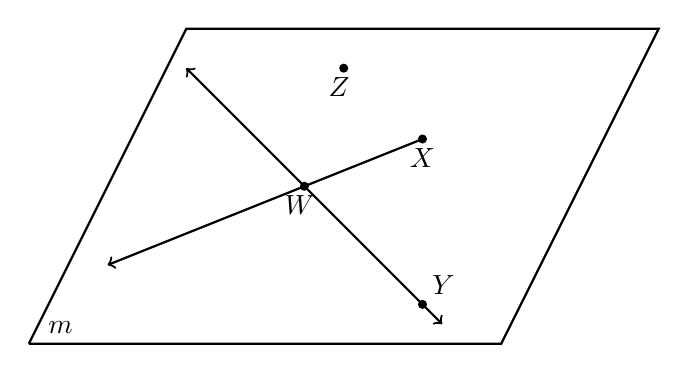
\begin{tikzpicture}
      \draw [thick](0,0) node[above right]{$\ m$} --(6,0)--(8,4)--(2,4)--(0,0);
      \draw [<-, thick] (1,1)--(5,2.6);
      \draw [fill] (4, 3.5) circle [radius=0.05] node[below]{$Z \ $};
      \draw [fill] (3.5,2) circle [radius=0.05] node[below]{$W \ $};
      \draw [fill] (5,2.6) circle [radius=0.05] node[below]{$X$};
      \draw [<->, thick] (2,3.5)--(5.25,.25);
      \draw [fill] (5,0.5) circle [radius=0.05] node[above right]{$Y \ $};
    \end{tikzpicture}
  \end{center}
\end{frame}

\begin{frame}{More definitions: intersections, coplanar}
Two lines \emph{intersect} if they cross. Their common point is the \emph{intersection}. 
(shown here, lines $j$ and $k$ intersect at point $P$)
\begin{center}
  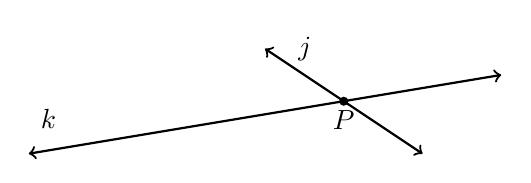
\begin{tikzpicture}
      \draw [<->, thick] (0,0)--(6,1);
      \draw [<->, thick] (3,1.333)--(5,0);
      \node at (0.25, 0.2)[above]{$k$};
      \node at (3.3, 1.333)[right]{$j$};
      \draw [fill] (4,0.666) circle [radius=0.05] node[below]{$P$};
    \end{tikzpicture}
  \end{center}
  \emph{Coplanar} means to lie in the same plane. Three points are always coplanar, but four points may not be.
  \begin{center}
    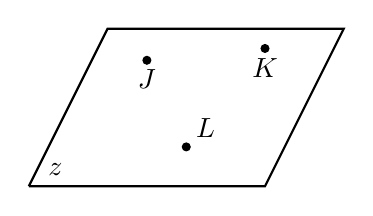
\begin{tikzpicture}[scale=1]
    \draw [thick](0,0) node[above right]{$\ z$} --(3,0)--(4,2)--(1,2)--(0,0);
    \draw [fill] (3,1.75) circle [radius=0.05] node[below]{$K$};
    \draw [fill] (1.5,1.6) circle [radius=0.05] node[below]{$J$};
    \draw [fill] (2,0.5) circle [radius=0.05] node[above right]{$L$};
  \end{tikzpicture}
\end{center}
\end{frame}

\section{1.4 Midpoint and bisector, 13 September}
\begin{frame}{Learning Target: I can \emph{bisect} a length}
  {CCSS: HSG.CO.A.1 Know precise geometric definitions  \hfill \alert{1.4 Monday 13 Sept}}
  
    \begin{block}{Do Now: Point $B$ is in the exact middle between $A$ and $C$}
      Given $AB=x+2$, $BC=11$. Find $x$.
        \begin{center}
          \begin{tikzpicture}
            \draw [fill] (0,0) circle [radius=0.05] node[below]{$A$};
            \draw [-, thick] (0,0)--(7,0);
            \draw [fill] (3.5,0) circle [radius=0.05] node[below]{$B$};
            \draw [fill] (7,0) circle [radius=0.05] node[below]{$C$};
            \node at (1.7,0.5) [above]{$x+2$};
            \node at (5.2,0.5) [above]{$11$};
          \end{tikzpicture}
        \end{center}
    \end{block}
    Hint: The line segment is split into two equal lengths. \vspace{3cm}
  \end{frame}

\begin{frame}{The \emph{midpoint} of a line segment}
    Given $\overline{ABC}$, with $AB=2x+2$, $AC=20$. $AB=BC$ \\[0.15in]
    Find $x$.
      \begin{center}
        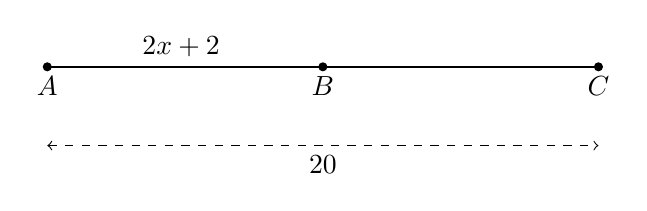
\begin{tikzpicture}
          \draw [fill] (0,0) circle [radius=0.05] node[below]{$A$};
          \draw [-, thick] (0,0)--(7,0);
          \draw [fill] (3.5,0) circle [radius=0.05] node[below]{$B$};
          \draw [fill] (7,0) circle [radius=0.05] node[below]{$C$};
          \node at (1.7,0) [above]{$2x+2$};
          %\node at (5.2,0) [above]{$?$};
          \draw [<->, dashed] (0,-1)--(7,-1);
          \node at (3.5,-1) [below]{$20$};
        \end{tikzpicture}
      \end{center} \vspace{2cm}
    \end{frame}

\begin{frame}{A \emph{bisector} creates two line segments with the same length}
  {\emph{Congruent} line segments are the same length}
  Given point $B$ is the midpoint of $\overline{AC}$, with $AB=x+7$, $BC=17$.
  Find $x$.
    \begin{center}
      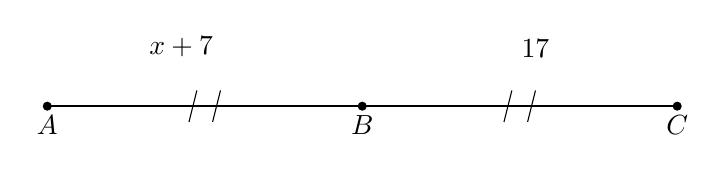
\begin{tikzpicture}
        \draw [fill] (0,0) circle [radius=0.05] node[below]{$A$};
        \draw [-, thick] (0,0)--(8,0);
        \draw [fill] (4,0) circle [radius=0.05] node[below]{$B$};
        \draw [fill] (8,0) circle [radius=0.05] node[below]{$C$};
        \node at (1.7,0.5) [above]{$x+7$};
        \node at (6.2,0.5) [above]{$17$};
        \draw (1.8,-0.2)--(1.9,0.2);
        \draw (2.1,-0.2)--(2.2,0.2);
        \draw (5.8,-0.2)--(5.9,0.2);
        \draw (6.1,-0.2)--(6.2,0.2);
      \end{tikzpicture}
    \end{center} \vspace{2cm}
    The \emph{midpoint} or \emph{bisector} of a line segment divides it exactly in half. \par \medskip
    \emph{Congruent} means equal in length, $\overline{AB} \cong \overline{BC}$ (also $AB=BC$)\par
    Mark congruent segments in diagrams with cross ``\emph{hash}" marks.
  \end{frame}

\begin{frame}{Review: Identifying objects in a plane}
  Circle or mark each item
  \begin{enumerate} 
    \item The point $H$
    \item The ray $\overrightarrow{JL}$
    \item The name of the plane shown
    \end{enumerate} \vspace{1cm}
    \begin{center}
      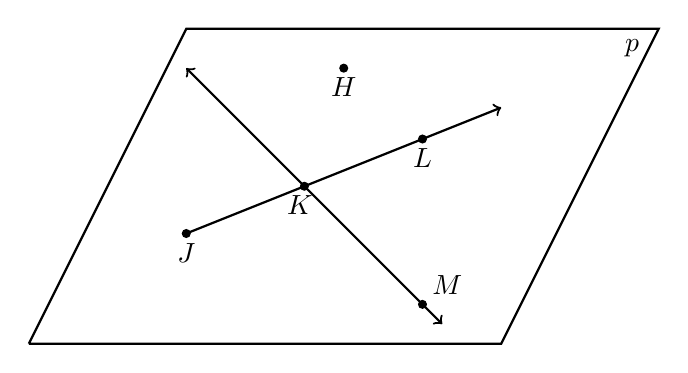
\begin{tikzpicture}
      \draw [thick](0,0)--(6,0)--(8,4) node[below left]{$p \ $} --(2,4)--(0,0);
      \draw [->, thick] (2, 1.4)--(6,3);
      \draw [fill] (4, 3.5) circle [radius=0.05] node[below]{$H$};
      \draw [fill] (2, 1.4) circle [radius=0.05] node[below]{$J$};
      \draw [fill] (3.5,2) circle [radius=0.05] node[below]{$K \ $};
      \draw [fill] (5,2.6) circle [radius=0.05] node[below]{$L$};
      \draw [<->, thick] (2,3.5)--(5.25,.25);
      \draw [fill] (5,0.5) circle [radius=0.05] node[above right]{$M \ $};
    \end{tikzpicture}
  \end{center}
\end{frame}


\section{1.5 Equilateral and isosceles triangles, perimeter \hfill 14 September}
\begin{frame}{Learning Target: I can work with objects having congruent parts}
  {CCSS: HSG.CO.A.1 Know precise geometric definitions  \hfill \alert{1.5 Wednesday 14 Sept}}
    \begin{block}{Do Now: Given $\overline{ST}$ with $S(-2)$ and $T(4)$}
      \begin{center}
              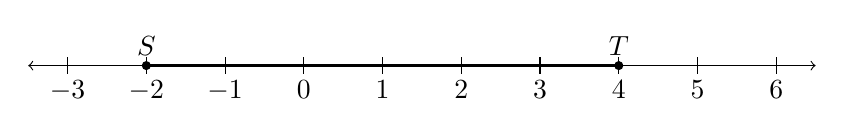
\begin{tikzpicture}
        \draw [<->] (-3.5,0)--(6.5,0);
        \draw [-, thick] (-2,0)--(4,0);
        \foreach \x in {-3,...,6} %2 leading for diff!=1
          \draw[shift={(\x,0)},color=black] (0pt,-3pt) -- (0pt,3pt) node[below=5pt]  {$\x$};
          \draw [fill] (-2,0) circle [radius=0.05] node[above] {$S$};
          \draw [fill] (4,0) circle [radius=0.05] node[above] {$T$};
      \end{tikzpicture}
      \end{center}
    What is the length of the segment $\overline{ST}$? Show your work as an equation.
    \end{block} \vspace{2cm}
    Lesson: Perimeter, congruent line segments in rectangles \& isosceles triangles
  \end{frame}

\begin{frame}{Negative number practice on a number line}
  {Take the difference in the points' values. Check by counting the marks.}
  Given $\overline{ST}$ with $S(-2)$ and $T(4)$, as shown on the number line.
  \begin{center}
     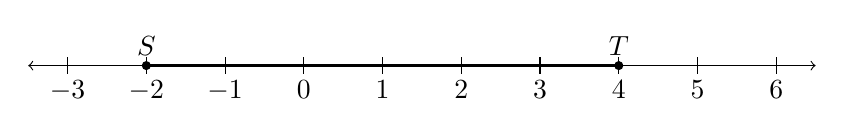
\begin{tikzpicture}
      \draw [<->] (-3.5,0)--(6.5,0);
      \draw [-, thick] (-2,0)--(4,0);
      \foreach \x in {-3,...,6} %2 leading for diff!=1
        \draw[shift={(\x,0)},color=black] (0pt,-3pt) -- (0pt,3pt) node[below=5pt]  {$\x$};
        \draw [fill] (-2,0) circle [radius=0.05] node[above] {$S$};
        \draw [fill] (4,0) circle [radius=0.05] node[above] {$T$};
    \end{tikzpicture}
  \end{center}
  What is the length of the segment $\overline{ST}$? Show your work as an equation.\par \vspace{3cm}
  Why is ``minus a negative" the same as add a positive? \vspace{2cm}  
\end{frame}

\begin{frame}{Use proper notation (including the bar over the letters)}
      Given $\triangle ABC$ write down two congruent line segments using proper notation.\\
        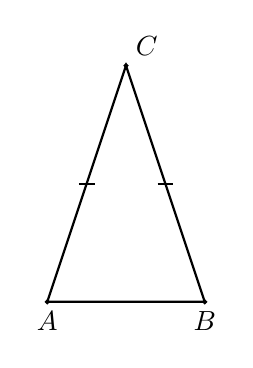
\begin{tikzpicture}[scale=0.5]
          \draw [thick](0,0)--(4,0)--(2,6)--(0,0);
          \draw [fill] (0,0) circle [radius=0.05] node[below]{$A$};
          \draw [fill] (4,0) circle [radius=0.05] node[below]{$B$};
          \draw [fill] (2,6) circle [radius=0.05] node[above right]{$C$};
          \draw [thick] (0.8,3)--(1.2,3); %tick mark
          \draw [thick] (2.8,3)--(3.2,3); %tick mark
        \end{tikzpicture}
      \end{frame}

\begin{frame}{On the diagram mark the congruent line segments with tick marks.}
      Given $\triangle STU$ with $\overline{ST} \cong \overline{TU}$. 
      \begin{center}
      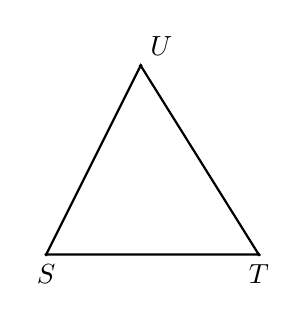
\begin{tikzpicture}[scale=0.3]
        \draw [thick](0,0)--(9,0)--(4,8)--(0,0);
        \draw [fill] (0,0) circle [radius=0.05] node[below]{$S$};
        \draw [fill] (9,0) circle [radius=0.05] node[below]{$T$};
        \draw [fill] (4,8) circle [radius=0.05] node[above right]{$U$};
      \end{tikzpicture}
      \end{center}
    \end{frame}

\begin{frame}{ Sketch an isosceles triangle}
  Mark the congruent sides with tick marks.\par \vspace{4cm}
  ToDo: equilateral $\triangle$, isosceles, perimeter, quadrilaterals
\end{frame}

\begin{frame}{Formal meanings of sketch, draw, and construct}
  \begin{enumerate}
    \item \emph{Sketch} is to make a freehand diagram of important features. \\[0.15cm]
    Use a pencil to write carefully in your notebook or on paper.  \smallskip
    \item \emph{Draw}  is to depict with accurate measures using ruler, protractor, and compass.\\[0.15cm]
    For example, draw a diagram of your room. \smallskip
    \item \emph{Construct} is a formal, logical process to create geometric figures using only a straightedge and compass. \smallskip
    \item Drawn to \emph{scale} means that all of the lengths are proportional. (e.g. a ``scale model'')\\[0.15cm]
    Tests will often warn that diagrams are ``not drawn to scale''
  \end{enumerate}
\end{frame}

\section{1.x Misc. review problems \hfill xx September}
\begin{frame}{Review problem slides}
  {CCSS: HSG.CO.A.1 Know precise geometric definitions  \hfill \alert{Review September}}
  Draw a ray. (careful! which direction does it go?)
  Given the points $X$ and $Y$, draw $\overrightarrow{YX}$.
  \vspace{2cm}
  \begin{center}
    \begin{tikzpicture}
    \draw [fill] (1,2) circle [radius=0.05] node[below]{$X$};
    \draw [fill] (5,0) circle [radius=0.05] node[below]{$Y$};
  \end{tikzpicture}
  \end{center} \vspace{1cm}
\end{frame}

\begin{frame}{Identify each item.}
  \begin{enumerate} 
    \item The point $A$
    \item The ray $\overrightarrow{BD}$
    \item The name of the plane
    \end{enumerate} \vspace{1cm}
    \begin{center}
      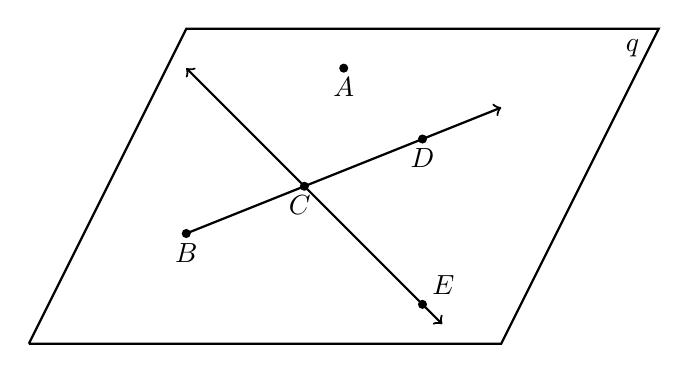
\begin{tikzpicture}
      \draw [thick](0,0)--(6,0)--(8,4) node[below left]{$q \ $} --(2,4)--(0,0);
      \draw [->, thick] (2, 1.4)--(6,3);
      \draw [fill] (4, 3.5) circle [radius=0.05] node[below]{$A$};
      \draw [fill] (2, 1.4) circle [radius=0.05] node[below]{$B$};
      \draw [fill] (3.5,2) circle [radius=0.05] node[below]{$C \ $};
      \draw [fill] (5,2.6) circle [radius=0.05] node[below]{$D$};
      \draw [<->, thick] (2,3.5)--(5.25,.25);
      \draw [fill] (5,0.5) circle [radius=0.05] node[above right]{$E \ $};
    \end{tikzpicture}
  \end{center}
\end{frame}

\begin{frame}{Apply the Segment Addition Postulate \\
  Show your work by marking the diagram and writing an equation.}
    Given $\overline{DEF}$, $DE=8.5$, and $EF=2.5$. Find ${DF}$.\\[0.75cm]
      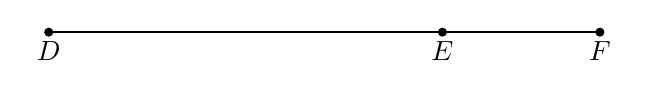
\begin{tikzpicture}
        \draw [-, thick] (0,0)--(7,0);
        \draw [fill] (0,0) circle [radius=0.05] node[below]{$D$};
        \draw [fill] (5,0) circle [radius=0.05] node[below]{$E$};
        \draw [fill] (7,0) circle [radius=0.05] node[below]{$F$};
      \end{tikzpicture} \vspace{4cm}
    \end{frame}

\begin{frame}{Find the length of the line segment $\overline{PQ}$.}
  Given $P(-2)$ and $Q(3)$, as shown on the number line. \\[0.25cm]
    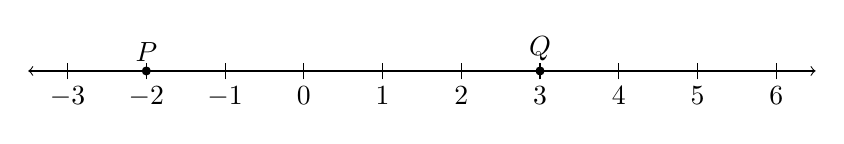
\begin{tikzpicture}
      \draw [<->] (-3.5,0)--(6.5,0);
      \draw [-, thick] (-2,0)--(3,0);
      \foreach \x in {-3,...,6} %2 leading for diff!=1
        \draw[shift={(\x,0)},color=black] (0pt,-3pt) -- (0pt,3pt) node[below=5pt]  {$\x$};
        \draw [fill] (-2,0) circle [radius=0.05] node[above] {$P$};
        \draw [fill] (3,0) circle [radius=0.05] node[above] {$Q$};
    \end{tikzpicture} \\
    State an equation and the solution. \\
Check your work by counting the distance. Leave marks to show your work. \vspace{5cm}  
\end{frame}

\begin{frame}{Segment addition practice}
  \begin{block}{Do Now: Given $\overline{LMN}$, $LM=3x+1$, $MN=7$, $LN=17$. Find ${x}$.}
    \begin{tikzpicture}
      \draw [-, thick] (0,0)--(7,0);
      \draw [fill] (0,0) circle [radius=0.05] node[below]{$L$};
      \draw [fill] (4,0) circle [radius=0.05] node[below]{$M$};
      \draw [fill] (7,0) circle [radius=0.05] node[below]{$N$};
      \node at (1.7,0) [above]{$3x+1$};
      \node at (5.5,0) [above]{$7$};
      \draw [<->, dashed] (0,-1)--(7,-1);
      \node at (3.5,-1) [below]{$17$};
    \end{tikzpicture} 
  \begin{enumerate}
    \item Write down an equation to represent the situation.
    \item Solve for $x$.
    \item Check your answer.
  \end{enumerate}
  \end{block}
\end{frame}
  
\begin{frame}{Solve for $x$ using the segment addition postulate}
  Given $\overline{LMN}$, $LM=3x+1$, $MN=7$, $LN=17$. Find ${x}$.\\[0.15in]
    \begin{tikzpicture}
      \draw [-, thick] (0,0)--(7,0);
      \draw [fill] (0,0) circle [radius=0.05] node[below]{$L$};
      \draw [fill] (4,0) circle [radius=0.05] node[below]{$M$};
      \draw [fill] (7,0) circle [radius=0.05] node[below]{$N$};
      \node at (1.7,0) [above]{$3x+1$};
      \node at (5.5,0) [above]{$7$};
      \draw [<->, dashed] (0,-1)--(7,-1);
      \node at (3.5,-1) [below]{$17$};
    \end{tikzpicture} %\vspace{1cm}
  \begin{enumerate}
    \item Write down an equation to represent the situation. \vspace{0.5cm}
    \item Solve for $x$. \vspace{2cm}
    \item Check your answer. \vspace{1cm}
  \end{enumerate}
\end{frame}

\begin{frame}{Midpoint example}
  \begin{block}{Given $M$ bisects $\overline{AB}$, $AM=5x+2$, $MB=20$.}
    \begin{enumerate}
      \item Mark the diagram with the values and tick marks
      \item Write an equation and solve for $x$
      \item Check your result
    \end{enumerate} \vspace{1cm}
      \begin{center}
        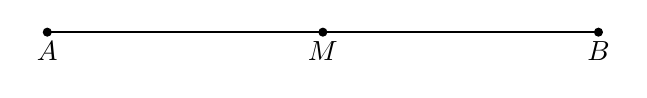
\begin{tikzpicture}
          \draw [fill] (0,0) circle [radius=0.05] node[below]{$A$};
          \draw [-, thick] (0,0)--(7,0);
          \draw [fill] (3.5,0) circle [radius=0.05] node[below]{$M$};
          \draw [fill] (7,0) circle [radius=0.05] node[below]{$B$};
          %\node at (1.7,0.5) [above]{$x+2$};
          %\node at (5.2,0.5) [above]{$11$};
          %\draw [<->, dashed] (0,-1)--(7,-1);
          %\node at (3.5,-1) [below]{$20$};
        \end{tikzpicture}
      \end{center}
  \end{block}
\end{frame}

\begin{frame}{Solve for $x$ given a bisector}
  Given $M$ is the midpoint of $\overline{AB}$, $AM=5x+2$, $MB=20$.
  \begin{enumerate}
    \item Mark the diagram with the values and tick marks
    \item Write an equation and solve for $x$
    \item Check your result
  \end{enumerate} \vspace{1cm}
    \begin{center}
      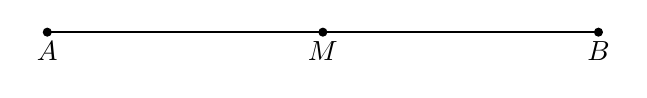
\begin{tikzpicture}
        \draw [fill] (0,0) circle [radius=0.05] node[below]{$A$};
        \draw [-, thick] (0,0)--(7,0);
        \draw [fill] (3.5,0) circle [radius=0.05] node[below]{$M$};
        \draw [fill] (7,0) circle [radius=0.05] node[below]{$B$};
        %\node at (1.7,0.5) [above]{$x+2$};
        %\node at (5.2,0.5) [above]{$11$};
        %\draw [<->, dashed] (0,-1)--(7,-1);
        %\node at (3.5,-1) [below]{$20$};
      \end{tikzpicture}
    \end{center} \vspace{4cm}
  \end{frame}

\begin{frame}{Segment addition with fractions}

  \begin{block}{Do Now: Given $\overline{RST}$, $RS=3 \frac{2}{3}$, and $RT=9 \frac{1}{3}$. Find ${ST}$.}\vspace{0.5cm}
      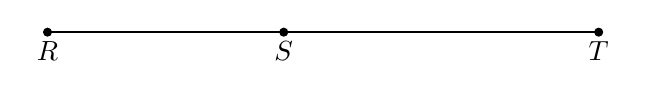
\begin{tikzpicture}
        \draw [-, thick] (0,0)--(7,0);
        \draw [fill] (0,0) circle [radius=0.05] node[below]{$R$};
        \draw [fill] (3,0) circle [radius=0.05] node[below]{$S$};
        \draw [fill] (7,0) circle [radius=0.05] node[below]{$T$};
      \end{tikzpicture}
  \end{block} \vspace{0.5cm}
\end{frame}

\begin{frame}{Mark the diagram and state your answer as a fraction}
    Given $\overline{RST}$, $RS=3 \frac{2}{3}$, and $RT=9 \frac{1}{3}$. Find ${ST}$.\\[0.75cm]
      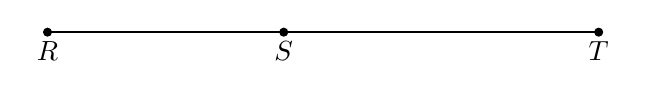
\begin{tikzpicture}
        \draw [-, thick] (0,0)--(7,0);
        \draw [fill] (0,0) circle [radius=0.05] node[below]{$R$};
        \draw [fill] (3,0) circle [radius=0.05] node[below]{$S$};
        \draw [fill] (7,0) circle [radius=0.05] node[below]{$T$};
      \end{tikzpicture} \\
      Solution \vspace{5cm} 
    \end{frame}
  
\begin{frame}{Segment bisector example}
  \begin{block}{Given $M$ bisects $\overline{PQ}$, $PM=x+7$, $PQ=23$.}
    \begin{enumerate}
      \item Mark the diagram with the values and tick marks
      \item Write an equation and solve for $x$
      \item Check your result
    \end{enumerate} \vspace{0.5cm}
      \begin{center}
        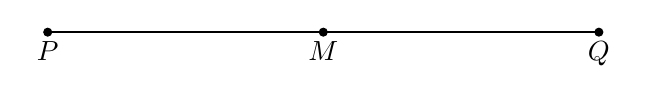
\begin{tikzpicture}
          \draw [fill] (0,0) circle [radius=0.05] node[below]{$P$};
          \draw [-, thick] (0,0)--(7,0);
          \draw [fill] (3.5,0) circle [radius=0.05] node[below]{$M$};
          \draw [fill] (7,0) circle [radius=0.05] node[below]{$Q$};
        \end{tikzpicture}
      \end{center}
  \end{block}
\end{frame}

\section{Sandbox}
\begin{frame}{Sandbox}
  \begin{enumerate}[(i)]
    \item one
    \item two
    \item three
  \end{enumerate}

  \fbox{box goes here \qquad xx \hspace{2cm} yy}

  \begin{enumerate}[T \quad F \,]
    \item one
    \item two
    \item three
  \end{enumerate}

  \begin{description}
    \item[End point] The point at the end of a line segments
    \item[Line] An infinite number of points extending in both directions forever 
  \end{description}

  \begin{definition}
    A \alert{prime number} is a number that has exactly two divisors. 
  \end{definition}
\end{frame}

\end{document}